\documentclass{beamer}

	\usepackage{datetime}
		\newdate{date}{04}{05}{2017}
	\usepackage[utf8]{inputenc}
		\usetheme{Darmstadt}
	\usepackage{graphicx}
	\graphicspath{{../fig/}}
	\usepackage{siunitx}
	\sisetup{separate-uncertainty}
	\usepackage{url}
	\usepackage{microtype}
	\usepackage[backend=bibtex,sorting=none,citestyle=authoryear,maxcitenames=1]{biblatex}
		\addbibresource{../bib/biblo} %Insert Bibliography file name
		\addbibresource{../bib/cust}
	\setlength\parindent{0pt}
	\usepackage{subcaption}
	\usepackage{float} 
	\usepackage{commath}
	\usepackage{amsfonts}
	\usepackage{booktabs}
	\setlength\heavyrulewidth{1.5pt}
	
	\usepackage[capitalise]{cleveref}
	\usepackage{pgfgantt}

%Information to be included in the title page:
\title{Machine Learning based simulation of Particle Physics Detectors}
\author{Seyon Sivarajah}

\date{\displaydate{date}}



\begin{document}
	
	\frame{\titlepage}
	\begin{frame}
		\frametitle{Overview}
		\tableofcontents
	\end{frame}
	
	\section{Detector Simulations}
	\label{sec:detsims}
	
		\begin{frame}
			\frametitle{Simulating events and detector response}
			\begin{figure}[H]
				\centering
				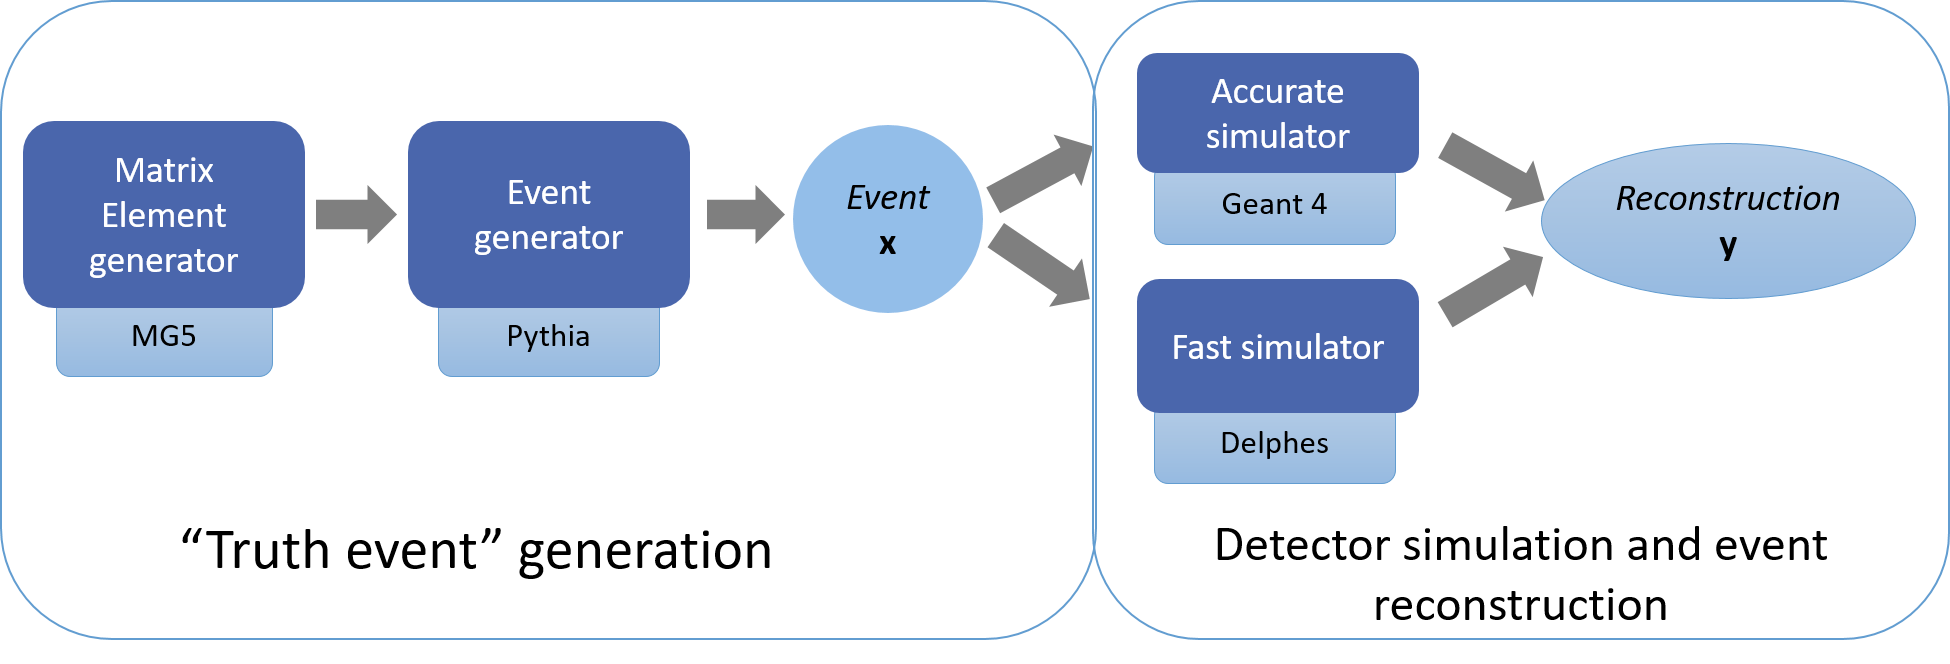
\includegraphics[width=1.0\linewidth]{simdiag}
				
				\caption{Summary of simulation process, from matrix element generation to final reconstruction from detector response.}
				\label{fig:simdiag}
			\alert{Project aim:} take steps towards a machine learning based fast simulation, training to replicate Delphes results. 
			\end{figure}
		\end{frame}
	
	\section{Machine Learning}
	\label{sec:gans}
		\begin{frame}
		\frametitle{Machine Learning}
		Traditional Machine learning:
		\begin{itemize}
			\item Classification 
			\item Regression
			\item Clustering
		\end{itemize} 
		\begin{block}{Generative Models}
			Learn from samples, $\mathbf{x}$, of a probability distribution $p(\mathbf{x})$, to produce accurate new members $\mathbf{y}$ by estimating $p(\mathbf{x})$. 
		\end{block}
		\end{frame}
	
		\begin{frame}
			\frametitle{Generative Adversarial Networks (GANS)}
			\begin{figure}[H]
				\centering
				\includegraphics[height=0.56\textheight]{goodgan}
				
				\caption{Generative Adversarial Nets process. Source: \textit{\autocite{GoodfellowNips}}}
				\label{fig:gandiag}
			
			\end{figure}
		
		$$
		\min_{G}\max_{D}V(D,G) = \mathbb{E}_{\mathbf{y}\sim p_{\text{data}}(\mathbf{y})} [\log(D(\mathbf{y})] + \mathbb{E}_{\mathbf{z}\sim p_{z}} [\log(1-D(G(z)))] 
		$$
		\end{frame}
	
		\begin{frame}
			\frametitle{Generative Adversarial Networks (GANs)}
			\begin{figure}[H]
				\centering
				\includegraphics[width=0.6\linewidth]{bedrooms}
				
				\caption{Generated bedroom image samples. Source: \textit{\autocite{GoodfellowNips}}}
				
			\end{figure}
		\end{frame}
	
	\section{Jet-images}
	\label{sec:jetims}
		\begin{frame}
			\frametitle{Jets to images}
			\begin{itemize}
				\item Jets: collimated hadronisation from high energy quark, gluon scattering.
				\item Image generation as prescribed by \textit{\cite{de2015jet}}.
				\item 2D in $\eta$, $\phi$ axes.
				\item Energy in calorimeter cell $\rightarrow$ pixel intensity.
			\end{itemize}
		\end{frame}
	
		\begin{frame}
			\frametitle{Signal and noise}
			 $W'$ boson from extensions to electroweak theory.
			 For example, $SU(2)_1 \times SU(2)_2 \times U(1)$ spontaneously broken to conventional electroweak. 
			 
			 $$
			 W' \rightarrow W + Z, \quad W \rightarrow q + q', \quad Z \rightarrow \nu + \bar{\nu}
			 $$
			 \begin{block}{}
			 	\centering
			 	Boosted W produces hadronic jet.
			 \end{block}
			 
			 "Noise" from generic quark and gluon jets.
		\end{frame}
	
		\begin{frame}
			\frametitle{Pre-processing}
			Based on facial recognition techniques \textit{\cite{cogan2014jet}}.
			\begin{enumerate}
				\item Trimming (anti-kT sub-jet clustering).
				\item Translation
				\item Rotation (cubic spline)
				\item Parity flip
			\end{enumerate}
		\end{frame}
		\begin{frame}
			\frametitle{Pre-processing}
			\begin{figure}[H]
				\centering
				\includegraphics[width=0.7\linewidth]{preproc}
			
				\label{fig:preproc}
				
			\end{figure}
		\end{frame}
	
		\begin{frame}
			\frametitle{Training image sample}
			\begin{figure}[H]
				\centering
				\includegraphics[width=0.75\linewidth]{ex_sig_real}
				
				\label{fig:ex_sig_real}
				
			\end{figure}
		\end{frame}
	
		\begin{frame}
			\frametitle{LAGAN}
			From \textit{\cite{de2017learning}}. Key components:
			\begin{itemize}
				\item Deep Convolutional (DCGAN) \textit{\autocite{Radford2015}}
				\item Auxillary Classifier (ACGAN) \textit{\autocite{odena2016conditional}}
				\item Locally Aware (LAGAN)
			\end{itemize}
			
		\end{frame}
	
		\begin{frame}
			\frametitle{LAGAN Architecture}
			\begin{figure}[H]
				\centering
				\includegraphics[width=0.8\linewidth]{laganarch}
				
				\caption{Generative Adversarial Nets process. Source: \textit{\cite{de2017learning}}}.
				\label{fig:lagan}
				
			\end{figure}
			
		\end{frame}


	
	\section{Generated Images}
	\label{sec:results}
	\begin{frame}
		\frametitle{Generated image sample}
		\begin{figure}[H]
			\centering
			\includegraphics[width=0.75\linewidth]{ex_sig_gen}
			
		\end{figure}
	\end{frame}
	
	\begin{frame}
		\frametitle{Average P+D Images}
		\begin{figure}[H]
			\centering
			\begin{subfigure}[t]{0.5\linewidth}
				\centering
				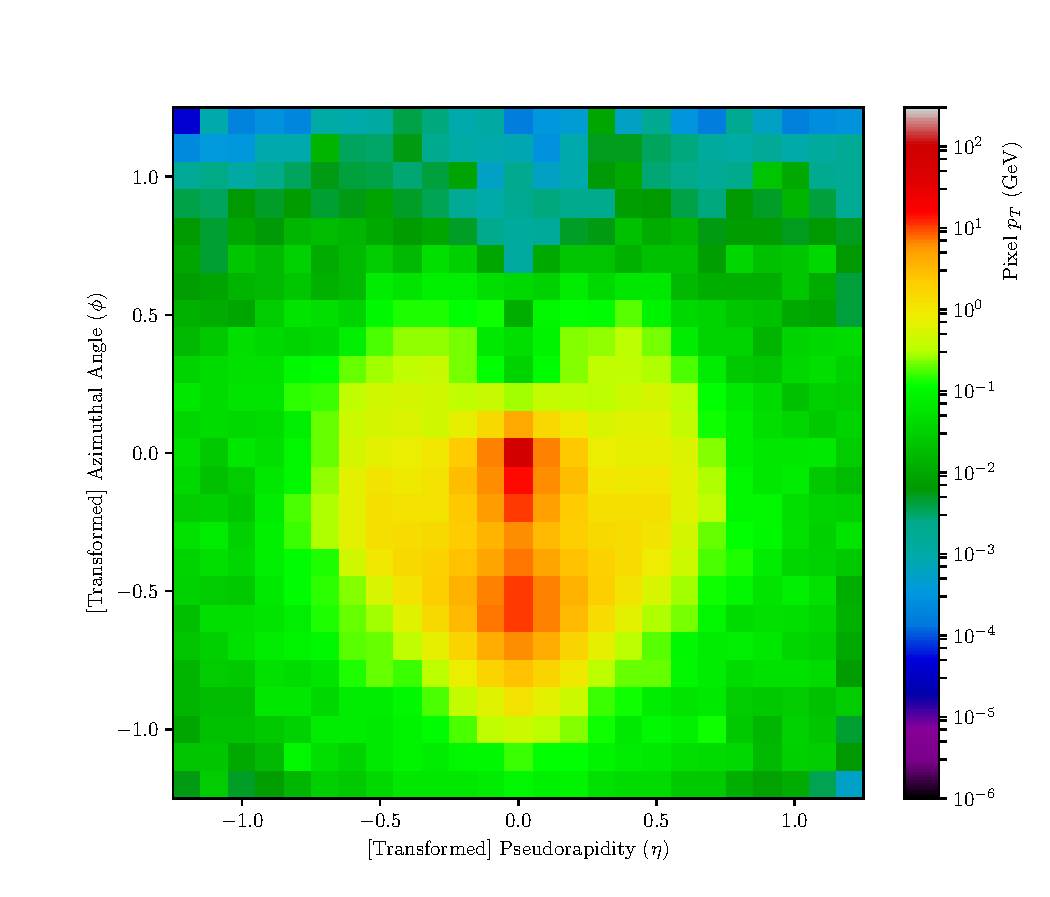
\includegraphics[width=1.0\linewidth]{av_sig_real_24k}
				\caption{$W'$ Signal}
			\end{subfigure}%
			~ 
			\begin{subfigure}[t]{0.5\linewidth}
				\centering
				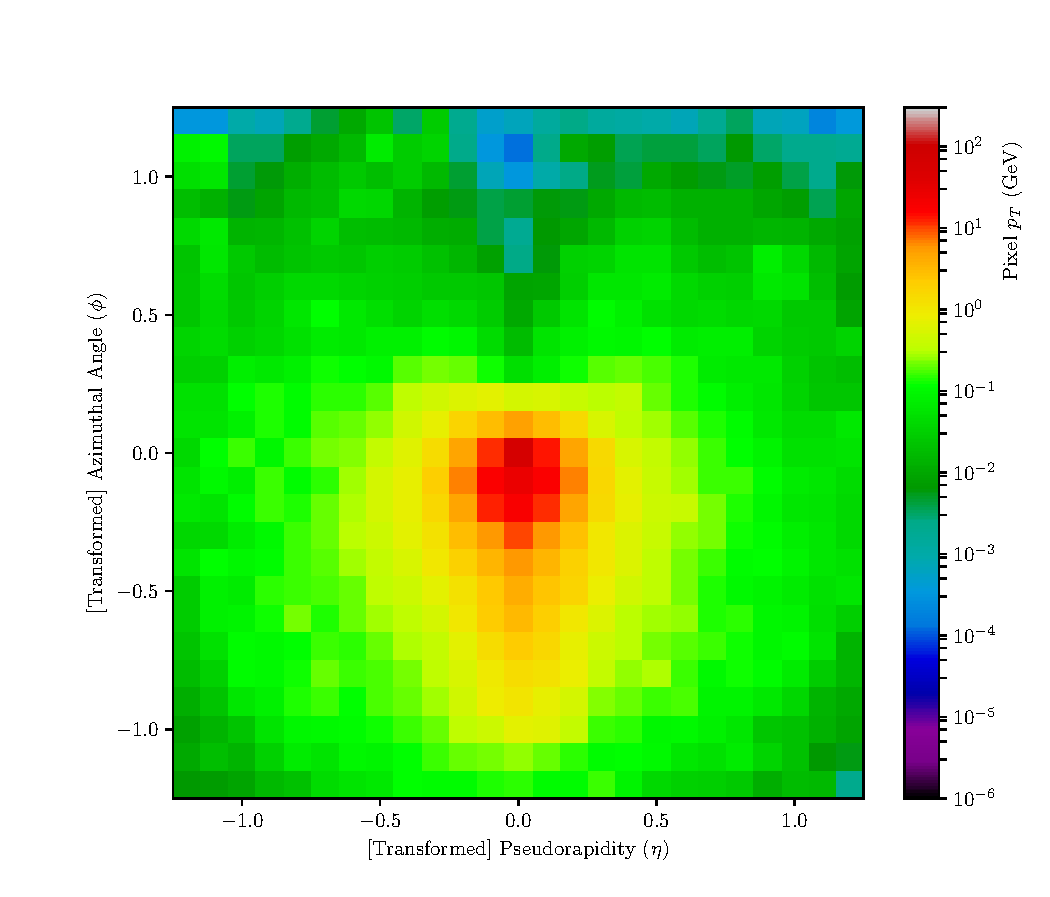
\includegraphics[width=1.0\linewidth]{av_noise_real_24k}
				\caption{QCD noise}
			\end{subfigure}


		\end{figure}
	\end{frame}

	\begin{frame}
		\frametitle{Average Generated Images}
		\begin{figure}[H]
			\centering
			\begin{subfigure}[t]{0.5\linewidth}
				\centering
				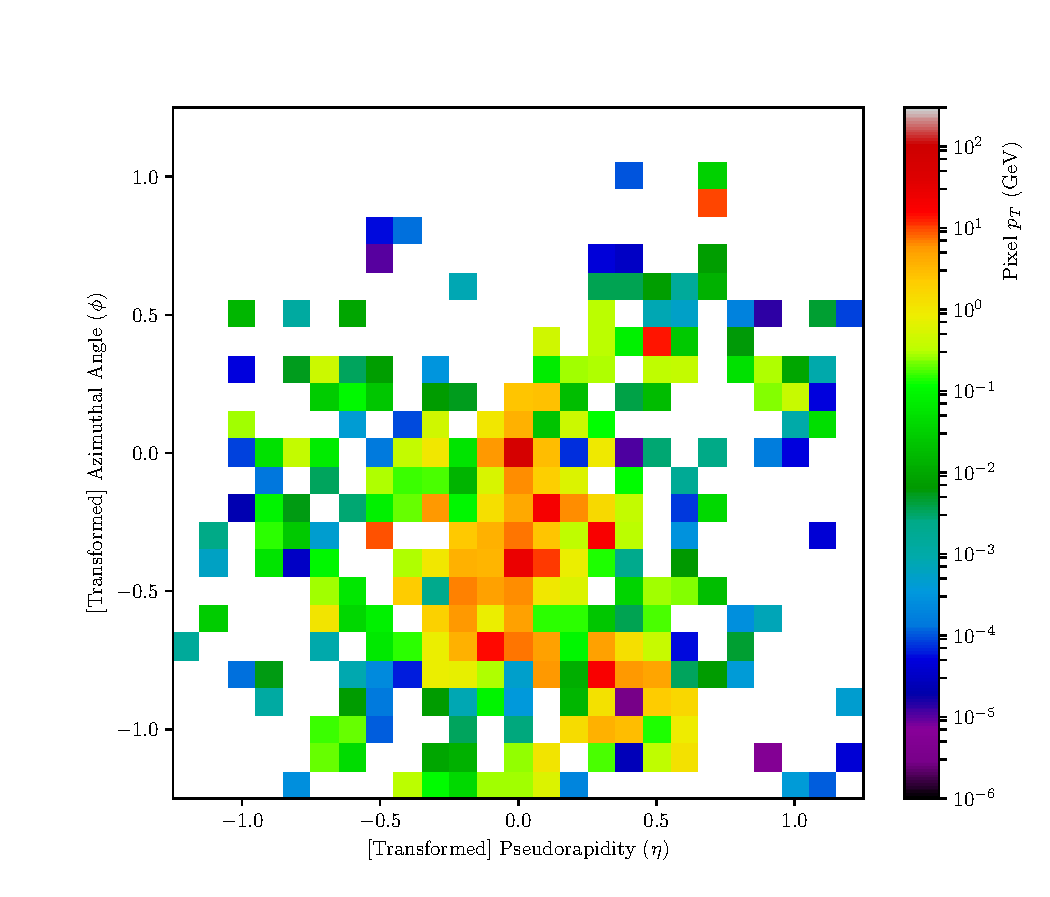
\includegraphics[width=1.0\linewidth]{av_sig_gen_24k}
				\caption{$W'$ Signal}
			\end{subfigure}%
			~ 
			\begin{subfigure}[t]{0.5\linewidth}
				\centering
				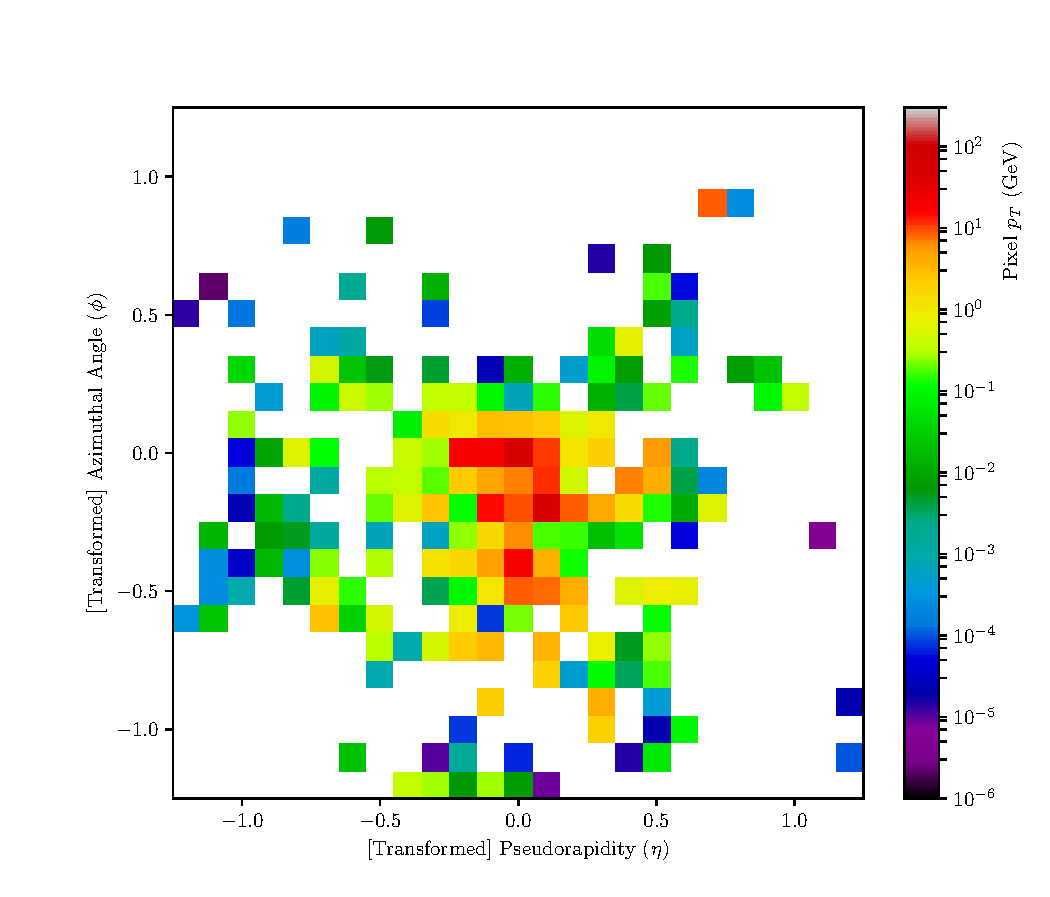
\includegraphics[width=1.0\linewidth]{av_noise_gen_24k}
				\caption{QCD noise}
			\end{subfigure}
			
			
		\end{figure}
	\end{frame}
	
	\begin{frame}
		\frametitle{Physical Distributions}
		For image $I$, with pixels indexed by $i$.
		$$
		m^2(I) = \bigg(\sum_i I_i\bigg)^2 -p^2_T(I) - \bigg(\sum_i I_i \sinh(\eta_i)\bigg)^2
		$$
		$$
		p_T^2(I) = \bigg(\sum_i I_i \cos(\phi_i)\bigg)^2 + \bigg(\sum_i I_i \sin(\phi_i)\bigg)^2
		$$
		
		
		$$
		\tau_n (I) \propto \sum_i I_i \min_a \bigg(\sqrt{(\eta_i - \eta_a)^2 + (\phi_i - \phi_a)^2}\bigg),
		$$
		
		$$
		\tau_{21} (I) = \tau_2 (I) / \tau_1 (I)
		$$
		$\eta_a$ and $\phi_a$ are axis values determined with the one-pass kt axis selection.
		
	\end{frame}
	
	\begin{frame}
		\frametitle{Mass}
		\begin{figure}[H]
			\centering
			\includegraphics[width=1\linewidth]{mass_comp}
			
		\end{figure}
	\end{frame}

	\begin{frame}
		\frametitle{Transverse Momentum}
		\begin{figure}[H]
			\centering
			\includegraphics[width=1\linewidth]{pt_comp}
			
		\end{figure}
	\end{frame}

	\begin{frame}
		\frametitle{N-subjettiness}
		\begin{figure}[H]
			\centering
			\includegraphics[width=1\linewidth]{tau21_comp}
			
		\end{figure}
	\end{frame}

	\begin{frame}
		\centering
		\frametitle{Speed Gains}
			\begin{tabular}{cc}
			\toprule Method  & Number of Events / sec \\
			\midrule Pythia+Delphes  & 41\\
			\midrule Generator  & 446\\

			\bottomrule
		\end{tabular}
	\end{frame}

	
	
	

	
	
	
\end{document}